%%%%%%%%%%%%%%%%%%%%%%%%%%%%%%%%%%%%%%%%
% Beamer Presentation
% LaTeX Template
% Version 1.0 (10/11/12)
%
% This template has been downloaded from:
% http://www.LaTeXTemplates.com
%
% License:
% CC BY-NC-SA 3.0 (http://creativecommons.org/licenses/by-nc-sa/3.0/)
%
%%%%%%%%%%%%%%%%%%%%%%%%%%%%%%%%%%%%%%%%%

% in R
% install.packages("tinytex")   
% require("tinytex")
% install_tinytex(force = TRUE)
% tlmgr_install('montserrat') 
% xelatex('Report.tex')

%----------------------------------------------------------------------------------------
%	PACKAGES AND THEMES
%----------------------------------------------------------------------------------------

\documentclass[10pt]{beamer}

\mode<presentation> {

% The Beamer class comes with a number of default slide themes
% which change the colors and layouts of slides. Below this is a list
% of all the themes, uncomment each in turn to see what they look like.

%\usetheme{default}
%\usetheme{AnnArbor}
%\usetheme{Antibes}
%\usetheme{Bergen}
%\usetheme{Berkeley}
%\usetheme{Berlin}
%\usetheme{Boadilla}
%\usetheme{CambridgeUS}
%\usetheme{Copenhagen}
%\usetheme{Darmstadt}
%\usetheme{Dresden}
%\usetheme{Frankfurt}
%\usetheme{Goettingen}
%\usetheme{Hannover}
%\usetheme{Ilmenau}
%\usetheme{JuanLesPins}
%\usetheme{Luebeck}
% \usetheme{Madrid}
%\usetheme{Malmoe}
%\usetheme{Marburg}
%\usetheme{Montpellier}
%\usetheme{PaloAlto}
%\usetheme{Pittsburgh}
%\usetheme{Rochester}
%\usetheme{Singapore}
\usetheme[
  bullet=circle,		% Other option: square
	shadow=false,			% Shading for beamer blocks
	]{Szeged}
%\usetheme{Warsaw}

% As well as themes, the Beamer class has a number of color themes
% for any slide theme. Uncomment each of these in turn to see how it
% changes the colors of your current slide theme.

%\usecolortheme{albatross}
%\usecolortheme{beaver}
%\usecolortheme{beetle}
%\usecolortheme{crane}
%\usecolortheme{dolphin}
%\usecolortheme{dove}
%\usecolortheme{fly}
%\usecolortheme{lily}
%\usecolortheme{orchid}
%\usecolortheme{rose}
%\usecolortheme{seagull}
%\usecolortheme{seahorse}
%\usecolortheme{whale}
%\usecolortheme{wolverine}

%\setbeamertemplate{footline} % To remove the footer line in all slides uncomment this line
%\setbeamertemplate{footline}[page number] % To replace the footer line in all slides with a simple slide count uncomment this line

%\setbeamertemplate{navigation symbols}{} % To remove the navigation symbols from the bottom of all slides uncomment this line
}

\usepackage{graphicx} % Allows including images
%\usepackege{subfig}
\usepackage{booktabs} % Allows the use of \toprule, \midrule and \bottomrule in tables

%----------------------------------------------------------------------------------------
%	TITLE PAGE
%----------------------------------------------------------------------------------------

\title[Resource selection studies with GLMMs]{Resource selection studies with marked animals: making inference to average selection with GLMMs} % The short title appears at the bottom of every slide, the full title is only on the title page

\author{Valentina La Morgia} % Your name
\institute[ISPRA] % Your institution as it will appear on the bottom of every slide, may be shorthand to save space
{
Istituto Superiore per la Protezione e la Ricerca Ambientale \\ % Your institution for the title page
\medskip
\textit{valentina.lamorgia@unito.it} % Your email address
}
\date{\today} % Date, can be changed to a custom date

\usepackage{Sweave}
\begin{document}

\Sconcordance{concordance:Slides1.tex:Slides1.Rnw:1 107 1 1 0 153 1 1 7 5 0 1 3 1 1 1 %
5 17 0 1 3 141 1 1 8 1 1 1 15 94 1 1 10 8 0 1 1 4 0 1 3 1 1 1 11 8 1 1 %
12 70 1 1 3 1 0 1 1 23 0 1 3 209 1 1 4 3 0 1 21 1 7 1 1 1 3 11 0 1 3 %
184 1 1 17 92 1}



\begin{frame}
\titlepage % Print the title page as the first slide
\end{frame}

%----------------------------------------------------------------------------------------
%	PRESENTATION SLIDES
%----------------------------------------------------------------------------------------


%------------------------------------------------
\section{Resource selection studies} % Sections can be created in order to organize your presentation into discrete blocks, all sections and subsections are automatically printed in the table of contents as an overview of the talk
%------------------------------------------------


\subsection{Motivation}

\begin{frame}
\frametitle{Motivation}

In the analysis of resource selection by animals, datasets are usually made up of a series of presence vs. (pseudo)absence data (binomial distribution)
% analizzare questo tipo di dati è di vitale importanza per molti motivi
\vspace{0.5cm}

\onslide<2->{

\begin{itemize}
\only<2>{
\item {\bf Adequate quantities of usable resources are necessary to sustain animal populations}.\\
The need to document the availability of resources is critical in efforts to preserve endangered species and manage exploited populations - {\it old growth forest is vital to the continued existence of the spotted owl (Strix occidentalis)?}
}
\only<3>{
\item Determining which resources (or conditions) are selected more often than others provides fundamental information about the nature of animals and how they meet their requirements for survival
}
\only<4>{
\item Differential resource selection is one of the principal relationships which permit species to coexist - {\it evaluation of the effect of domestic animals on wild animal forage}
}
\onslide<5>{
\item The process of natural selection can occur when resource selectivity results in
 successful (e.g., breeding) and unsuccessful individuals - {\it food and oviposition selection play a significant role in evolution and speciation among some insects}
}
\end{itemize}
}

% Gli ecologi sono da sempre interessati alla resource selection... analisi autoecologica per eccellenza
% Lo dimostrano tutti gli sforzi fatti per misurare in qualche modo la selezione dell'habitat da parte degli animali (o la scelta del cibo, ad esempio)

\end{frame}

%------------------------------------------------
\subsection{Definitions}
\begin{frame}
\frametitle{Basic concepts}

It is often assumed that a species will select
resources that are best able to satisfy its life requirements, and that high quality
resources will be selected more than low quality ones.\\
\vspace{0.5cm}
The availability of various
resources is not generally uniform in nature, and use may change as availability
changes.\\
\vspace{0.5cm}
Therefore, {\it used resources should be compared to available (or unused)
resources} in order to reach valid conclusions concerning resource selection.

\end{frame}

%------------------------------------------------
\begin{frame}
\frametitle{Definitions}


\begin{block}{Usage}
The usage of a resource is defined as that quantity of the resource that is utilized
by an animal (or population of animals) in a fixed period of time.
\end{block}

\begin{block}{Abundance and availability}
The abundance of a resource is the quantity of the resource in the environment.\\
The availability of
a resource is the quantity accessible to the animal (or population of animals) during that
same period of time.
\end{block}

\begin{block}{Selection and preference}
When
resources are used disproportionately to their availability, use is said to be selective.\\
Selection is the process in which an animal chooses a resource, and
preference is the likelihood that a resource will be selected if offered on an equal basis
with others.
\end{block}

% ok, we have definitions, concepts, we know the data type and we have a tool... what's next?

\end{frame}


%------------------------------------------------

\section{Case study}
\subsection{Case study description}

\begin{frame}
\frametitle{A case study}

\begin{figure}
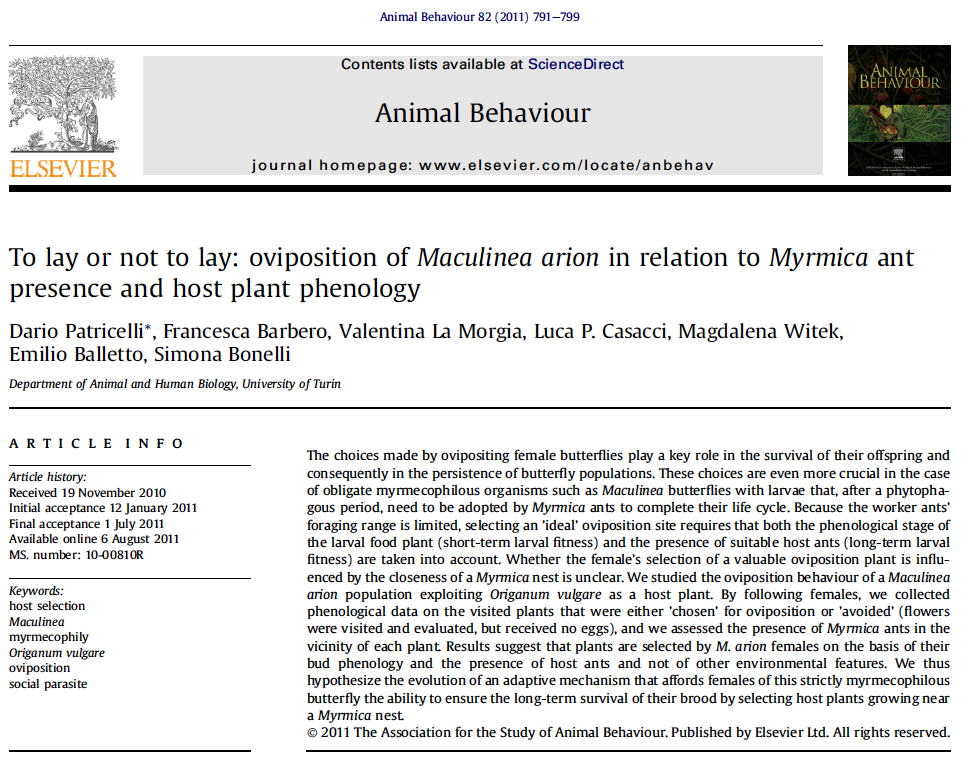
\includegraphics[width=0.8\linewidth]{pictures/casestudy}
\end{figure}


\end{frame}



%------------------------------------------------
\begin{frame}
\frametitle{A case study}

\begin{columns}

\column{.4\textwidth}
\begin{figure}
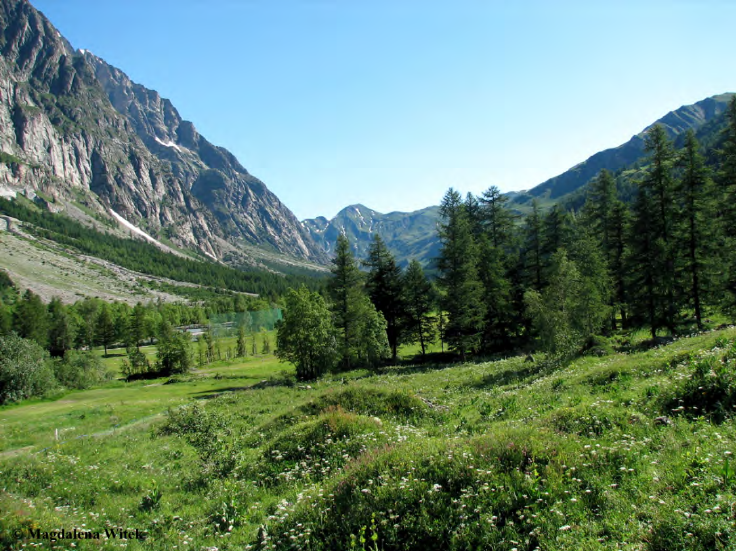
\includegraphics[width=0.9\linewidth]{pictures/studyarea}
\end{figure}
\vspace{2.5cm}
.

\column{.5\textwidth}
\begin{center}
\begin{figure}
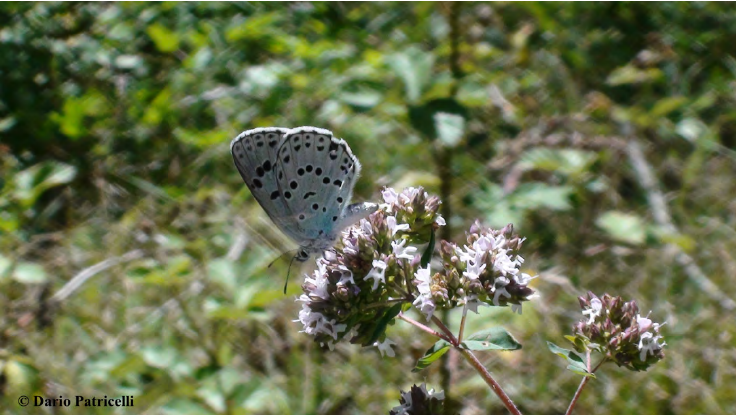
\includegraphics[width=.85\linewidth]{pictures/Maculineaarion}
\end{figure}


\begin{figure}
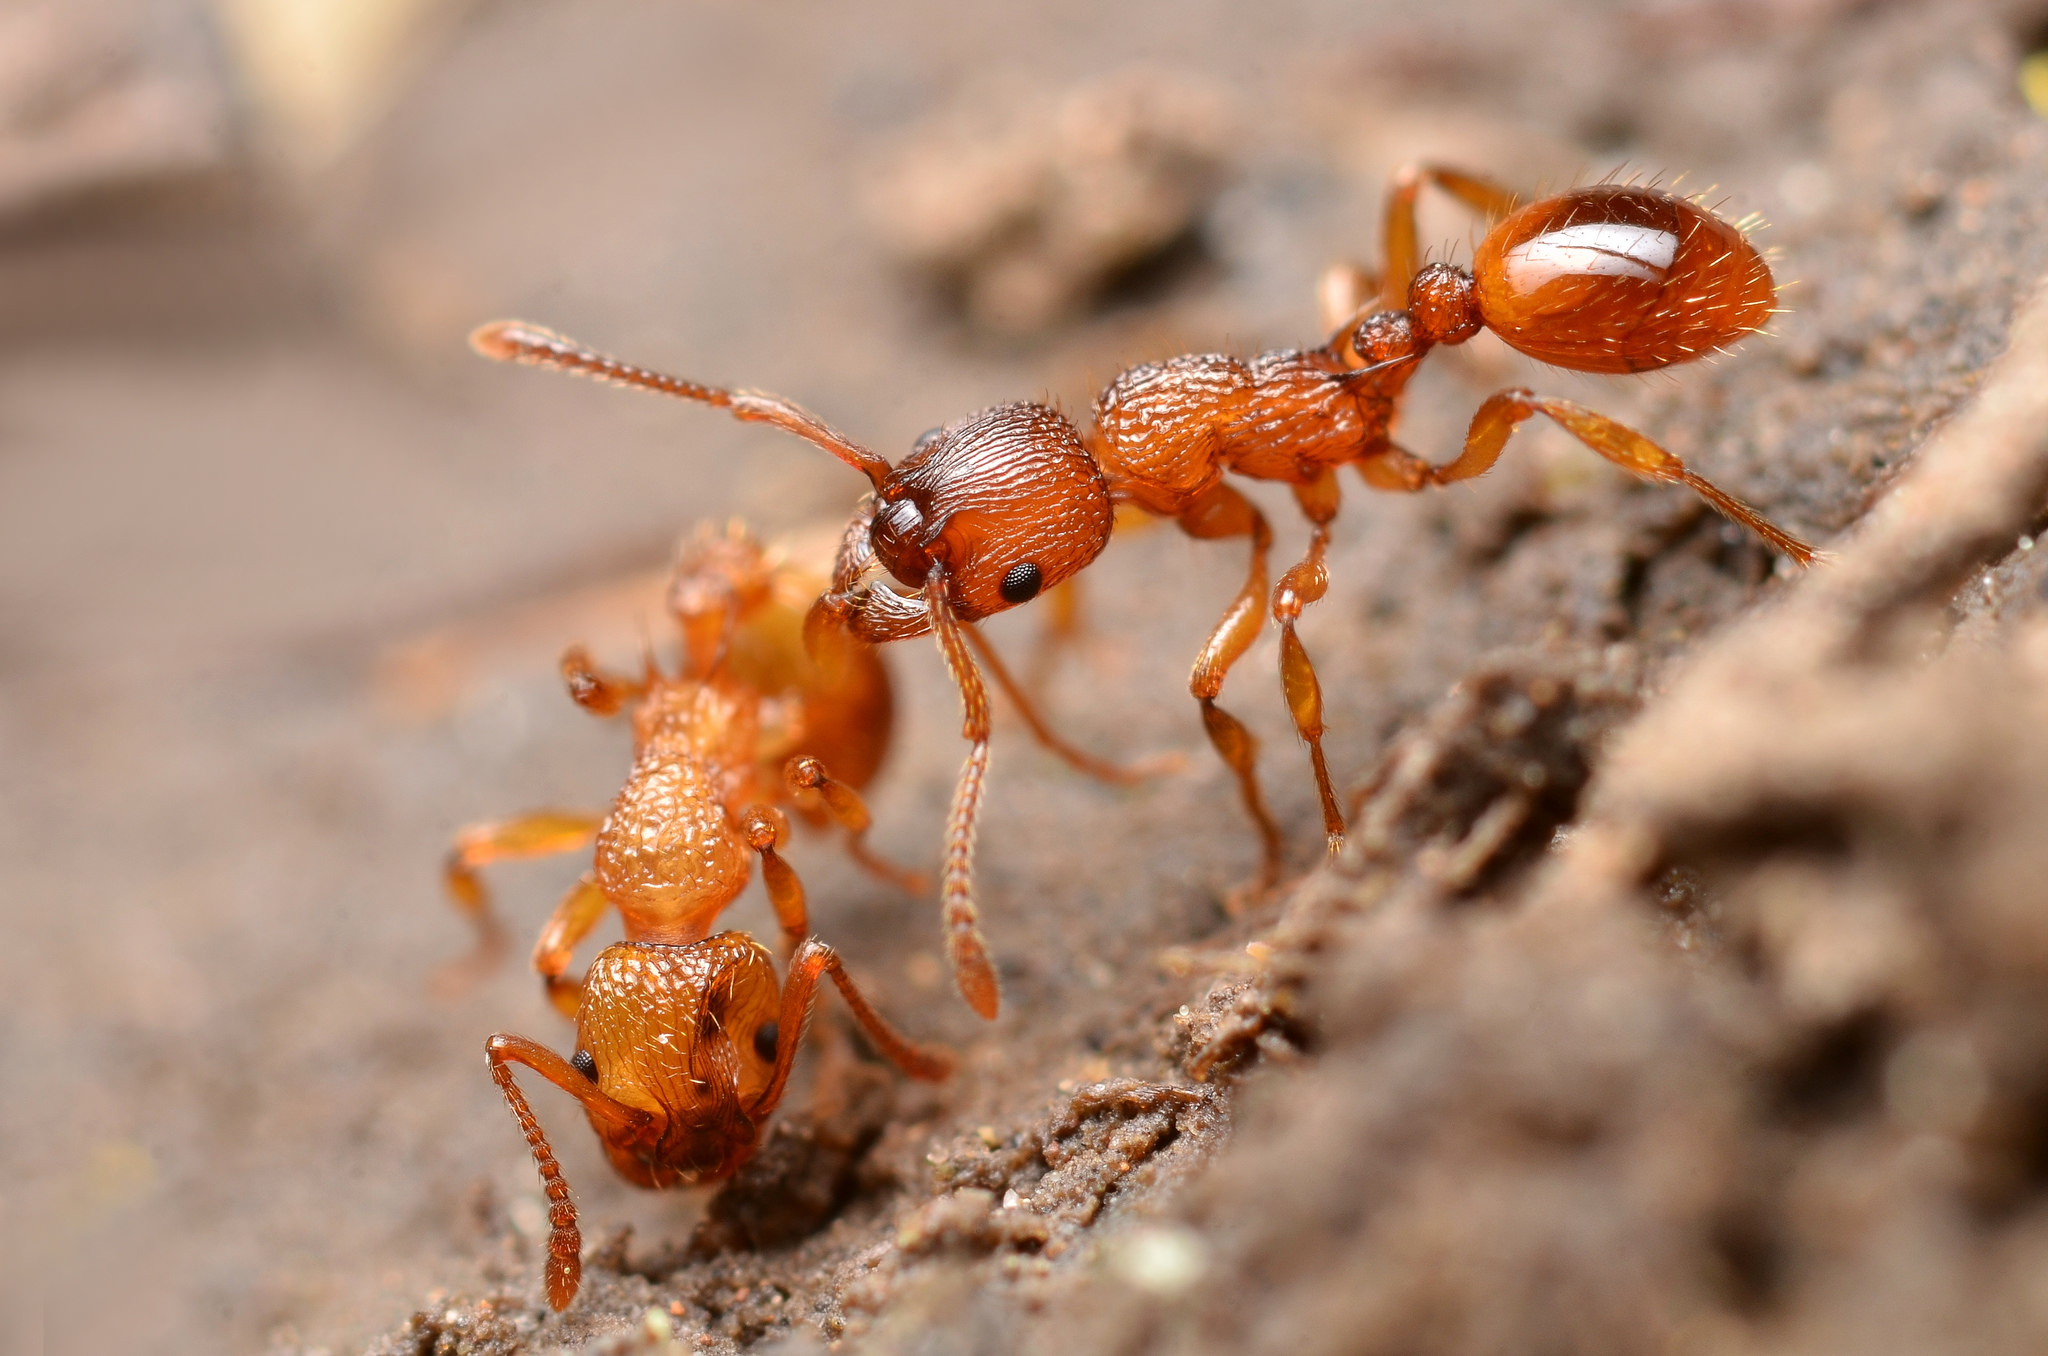
\includegraphics[width=.85\linewidth]{pictures/Myrmica}
\end{figure}
\end{center}

\end{columns}

\end{frame}

%------------------------------------------------

\subsection{Study design}
\begin{frame}[fragile]
\frametitle{Data}


\begin{Schunk}
\begin{Soutput}
 1  2  3  4  5  6  7  8  9 10 12 13 14 15 16 17 18 19 20 21 22 23 
 4  2  5  9  9 12 13 19  3 27 31 10 12  2  5  9  9  2  7 17  4  3 
\end{Soutput}
\end{Schunk}


\begin{Schunk}
\begin{Soutput}
'data.frame':	214 obs. of  13 variables:
 $ X                   : int  1 2 3 4 5 6 7 8 9 10 ...
 $ id                  : int  1 2 3 4 5 6 7 8 9 10 ...
 $ Egg10               : int  0 0 0 0 0 0 0 0 0 0 ...
 $ MyrmicaYN           : int  0 0 0 0 0 0 0 0 0 0 ...
 $ Noperaiepittfall    : int  0 0 0 0 0 0 0 0 0 0 ...
 $ Horigano            : num  50 50 30 60 70 37.5 50 45 25 55 ...
 $ HGrass              : int  10 10 10 40 15 15 10 15 15 5 ...
 $ Origanupatchdiameter: int  50 50 3 60 190 50 120 90 15 25 ...
 $ BV                  : int  0 0 1 1 1 0 1 1 1 1 ...
 $ BVR                 : int  0 0 0 0 0 0 0 0 0 0 ...
 $ BR                  : int  1 1 0 0 0 1 0 0 0 0 ...
 $ BF                  : int  1 1 0 0 0 1 0 0 0 0 ...
 $ NB                  : int  0 0 0 0 0 0 1 0 1 0 ...
\end{Soutput}
\end{Schunk}


\end{frame}



%------------------------------------------------
\begin{frame}
\frametitle{Study design}

% \begin{figure}
% 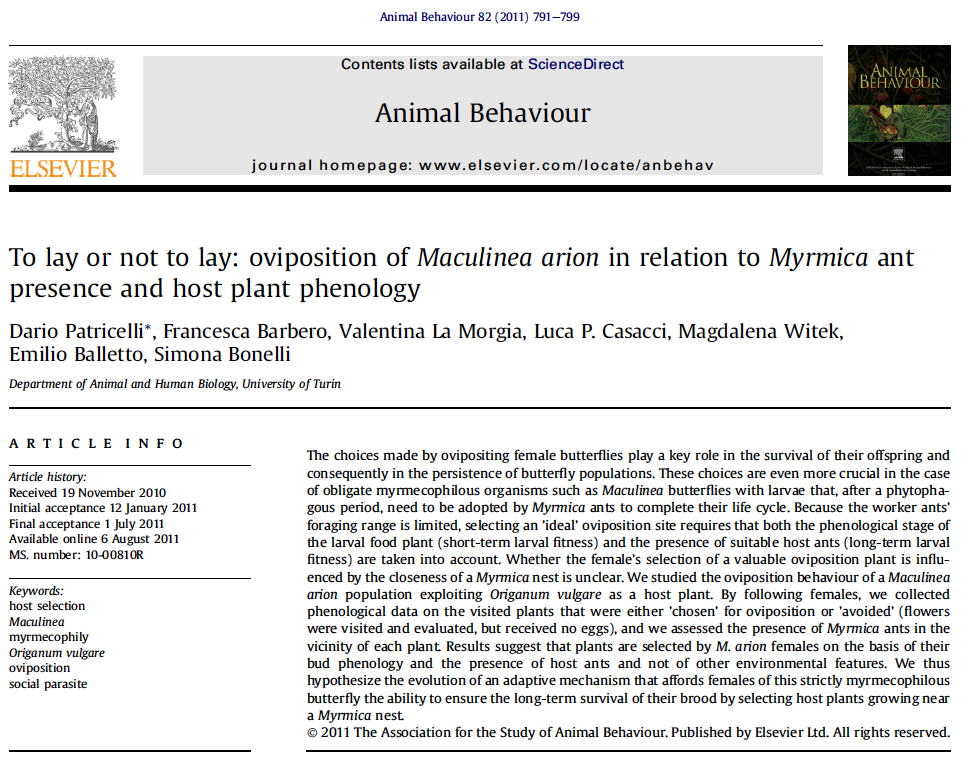
\includegraphics[width=0.8\linewidth]{pictures/casestudy}
% \end{figure}
Three general study designs for evaluating resource selection have been identified in the literature - they differ with respect to the level at which resource use and availability are measured, at the population level or for each animal.\\

% \onslide<2->{
\begin{block}{Design I}
Measurement are made at the population level. Individual animals are not identified.
\end{block}
% }

% \onslide<3->{
\begin{block}{Design II}
Individual animals are identified and the use of resources is measured for each, but availability is measured at the population level.
\end{block}
% }

% \onslide<4->{
\begin{block}{Design III}
Individual animals are identified and both the use of resources and their availability are measured for each marked animal.
\end{block}
% }

\end{frame}

%------------------------------------------------

\section{Generalized Linear Model}
\subsection{Data exploration}

\begin{frame}[fragile]
\frametitle{Data exploration - exercise 1}

% We define an outlier as an observation that has a
% relatively large or small value compared to the majority of
% observations.
% 
% <<datiglm-summary, echo=FALSE>>=
% 
% summary(dati.glm[,c("Noperaiepittfall","Horigano","HGrass")])
% 
% @
% 
% % l'analisi degli outlier non è rilevante per le variabili binomiali (es. Egg10, BV)
% % ma lo è per il numero di formiche, per l'altezza delle piante, dell'erba e del diametro delle piante
% \end{frame}
% 
% 
% %------------------------------------------------
% \begin{frame}[fragile]
% \frametitle{Step 1: Are there outliers in Y and X?}
% 
% <<label=datiglm-boxplot, fig=TRUE, include=FALSE, echo=FALSE>>=
% 
% boxplot(dati.glm[,c("Noperaiepittfall",
%                     "Horigano","HGrass",
%                     "Origanupatchdiameter")])
% 
% @
% 
% \begin{figure}
% 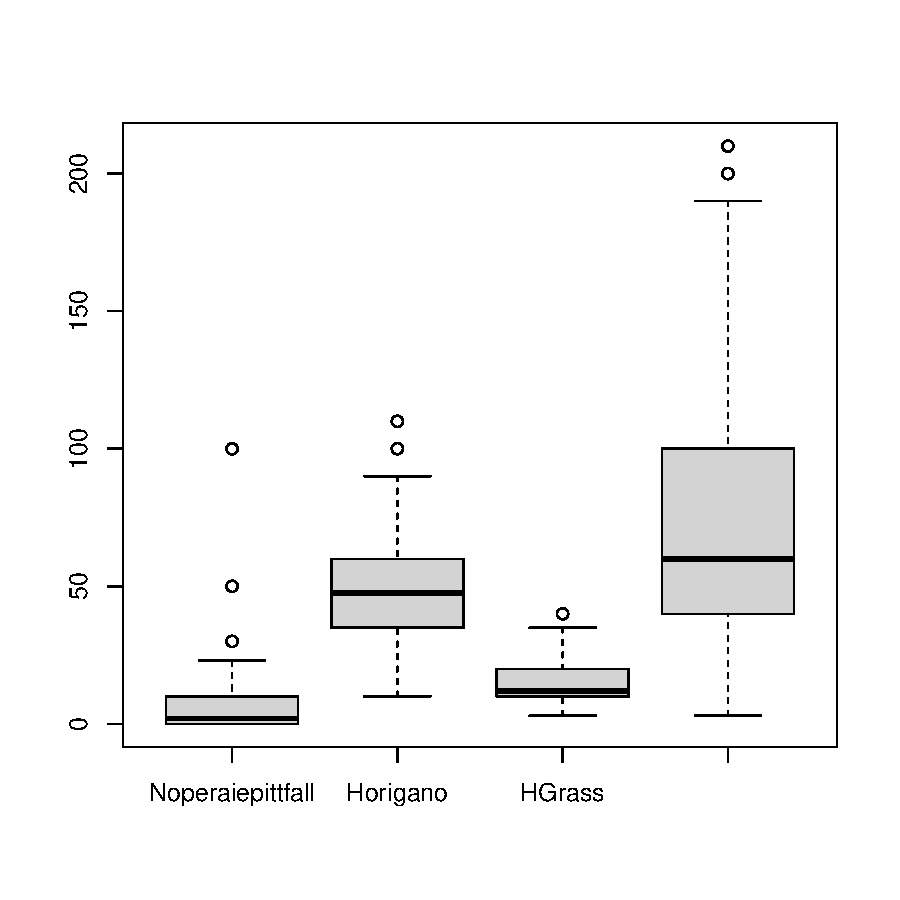
\includegraphics[width=0.6\textwidth]{pictures/Rplot-datiglm-boxplot.pdf}
% \end{figure}
% 
% \end{frame}
% 
% 
% %------------------------------------------------
% \begin{frame}[fragile]
% \frametitle{Step 1: Are there outliers in Y and X?}
% 
% <<label=datiglm-dotchart, fig=TRUE, include=FALSE, echo=FALSE>>=
% 
% op <- par(mfrow=c(1,4))
% dotchart(dati.glm$Noperaiepittfall, main="Noperaiepittfall")
% dotchart(dati.glm$Horigano, main="Horigano")
% dotchart(dati.glm$HGrass, main="HGrass")
% dotchart(dati.glm$Origanupatchdiameter, main="Origanupatchdiameter")
% par(op)
% 
% @
% 
% \begin{figure}
% 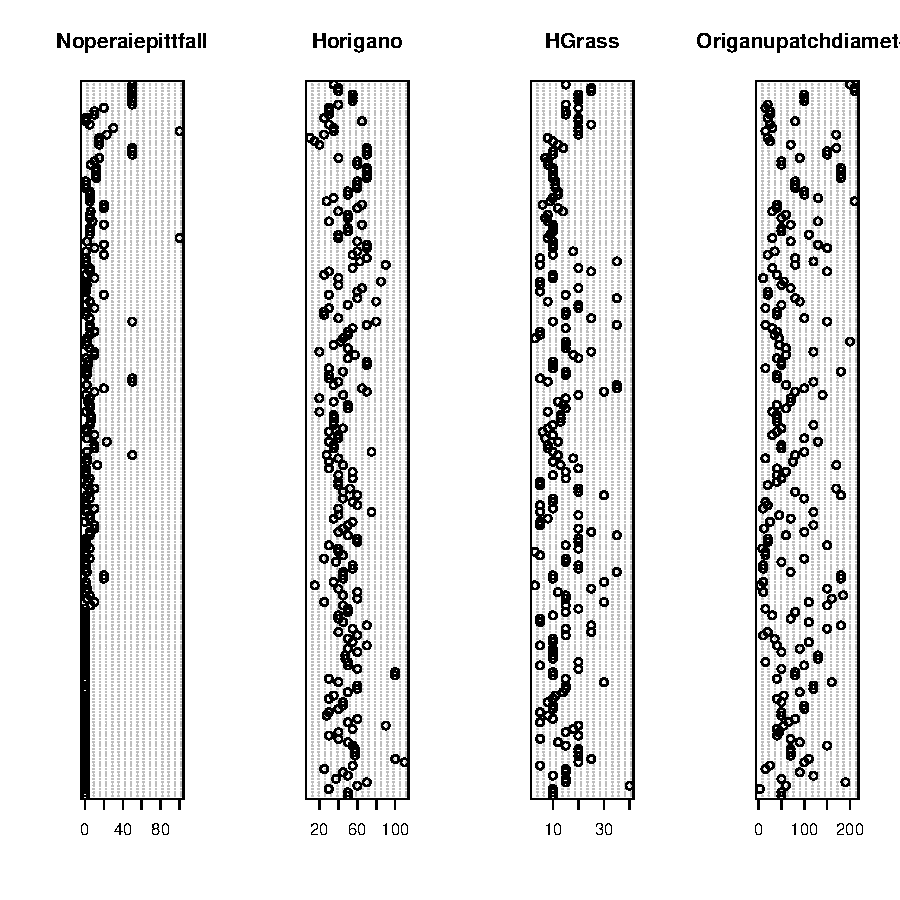
\includegraphics[width=0.6\textwidth]{pictures/Rplot-datiglm-dotchart.pdf}
% \end{figure}
% % identifico in particolare due outlier per quanto riguarda il numero di formiche, ma lo lascio perché ha un significato biologico
% 
% \end{frame}
% 
% 
% %------------------------------------------------
% % \begin{frame}
% % \frametitle{Step 2: Do we have homogeneity of variance?}
% % 
% % In regression-type models, verification of homogeneity
% % should be done using the residuals of the model; i.e. by plotting
% % residuals vs. fitted values, and making a similar set of conditional
% % boxplots for the residuals. In all these graphs the residual
% % variation should be similar. The solution to heterogeneity of
% % variance is either a transformation of the response variable to
% % stabilize the variance, or applying statistical techniques that
% % do not require homogeneity (e.g. generalized least squares).\\
% % 
% % For linear regression, the ratio between the largest and smallest variance should be < 4.
% % 
% % \end{frame}
% 
% %------------------------------------------------
% % \begin{frame}[fragile]
% % \frametitle{Step 3: Are the data normally distributed?}
% % 
% % It does not apply!!
% % 
% % \end{frame}
% 
% %------------------------------------------------
% \begin{frame}[fragile]
% \frametitle{Step 4: Are there lots of zeros in the data?}
% 
% <<label=datiglm-zeroonetable>>=
% 
% table(dati.glm$Egg10)
% 
% @
% 
% 
% \end{frame}
% 
% %------------------------------------------------
% \begin{frame}[fragile]
% \frametitle{Step 5: Is there collinearity among the covariates?}




\begin{figure}
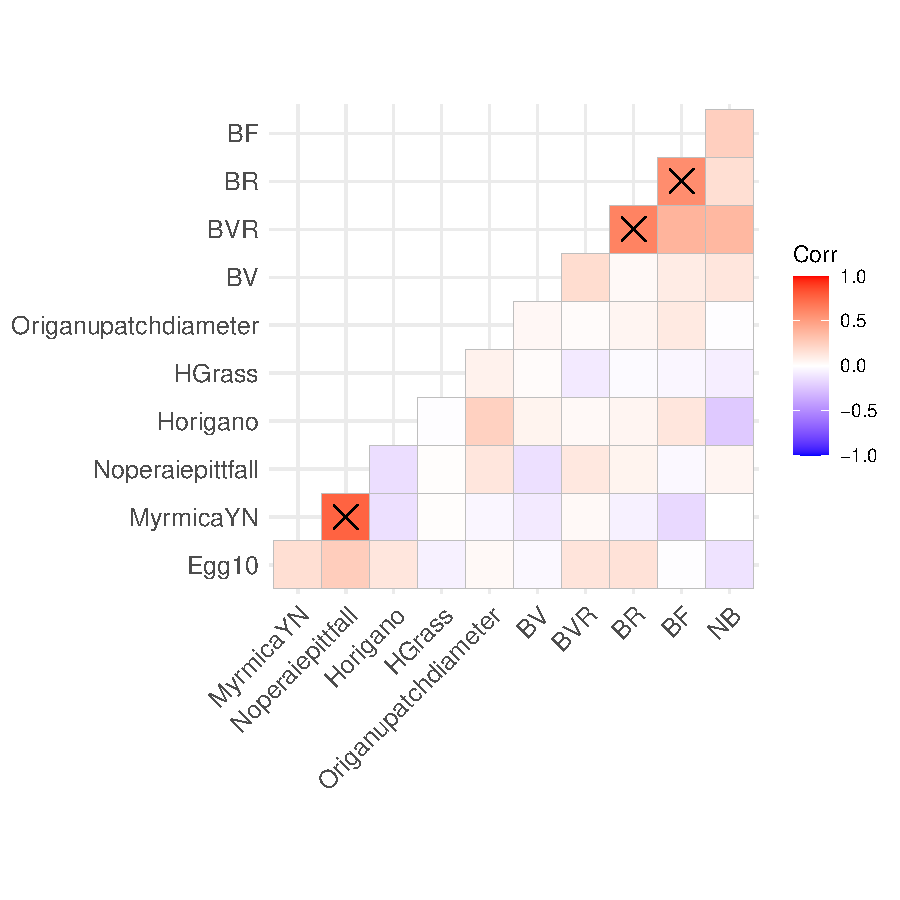
\includegraphics[width=0.8\textwidth]{pictures/Rplot-datiglm-correlazioni2.pdf}
\end{figure}
% # l'analisi delle correlazioni indica che: o metto MyrmicaYN o NoperaiepittfallS
% # BVR è correlato con BR
% # BR è correlato con BVR e con BF
% 
% # tolgo BR

\end{frame}


%' %------------------------------------------------
%' \begin{frame}[fragile]
%' \frametitle{Step 6: What are the relationships between Y and X variables?}
%' 
%' <<label=datiglm-relazioniXY, fig=TRUE, include=FALSE, echo=FALSE, eval=FALSE>>=
%' 
%' My.xy.plot <- function(AllY, AllX, ID) {
%'   library(lattice)
%'   library(mgcv)
%'   Z <- xyplot(AllY ~ AllX|ID, col = 1,
%'               xlab = "Explanatory variables",
%'               ylab = "Response variable",
%'               strip = function(bg='white', ...)
%'                 strip.default(bg='white', ...),
%'               scales = list(alternating = T,
%'                             x = list(relation = "free"),
%'                             y = list(relation = "free")),
%'               panel=function(x, y){
%'                 panel.grid(h=-1, v= 2)
%'                 panel.abline(0,0)
%'                 panel.points(x, y, col = 1)
%'                 panel.loess(x, y, col = 1, lwd = 2)
%'               })
%'   print(Z)
%' }
%' 
%' Y    <- dati.glm$Egg10
%' MyX  <- names(dati.glm[,-c(1,2)])
%' X    <- dati.glm[, MyX]
%' 
%' # keep it as it is
%' AllX <- as.vector(as.matrix(X))
%' ID   <- rep(MyX, each = length(Y))
%' AllY <- rep(Y, length(MyX))
%' My.xy.plot(AllY, AllX, factor(ID))     #call the function created above
%' 
%' @
%' 
%' % NON LO FACCIO PERCHé GRAFICI DI DIFFICILE INTERPRETAZIONE PER VARIABILE 0/1
%' % INOLTRE L'ASSENZA DI RELAZIONI A COPPIE NON SIGNIFICA CHE POI NON POSSANO EMERGERE RELAZIONI SIGNIFICATIVE NELLA REGRESSIONE MULTIPLA
%' 
%' 
%' 
%' %------------------------------------------------
%' \begin{frame}[fragile]
%' \frametitle{Step 7: Should we consider interactions?}
%' 
%' <<label=datiglm-interactions, fig=TRUE, include=FALSE, echo=FALSE, eval=FALSE>>=
%' 
%' #E Interactions
%' coplot((N ~ LOGAREAV | Cat),
%'        data = Birds1)
%' 
%' 
%' coplot(N ~ LOGAREAV | Cat,
%'        data = Birds1,
%'        panel = function(x, y, ...) {
%'          tmp <- lm(y ~ x, na.action = na.omit)
%'          abline(tmp)
%'          points(x, y) })
%' 
%' @
%' 
%' \end{frame}


%------------------------------------------------

%\section{Generalized Linear Model}
\subsection{Model fitting and selection}



%------------------------------------------------
\begin{frame}[fragile]
\frametitle{Model fitting: the base model - exercise 2}


We use a typical fixed-effects exponential resource selection function:
$$ \hat{w}(x) = exp(\hat{\beta}_0 + \hat{\beta}_1 x_1 + \hat{\beta}_2 x_2 + ... + \hat{\beta}_n x_n) $$ 
Parameters are estimated from logistic regression

\begin{Schunk}
\begin{Sinput}
> # names(dati.glm)
> mod.glm <- glm(Egg10 ~ Noperaiepittfall + 
+                  Horigano + HGrass + 
+                  Origanupatchdiameter + 
+                  factor(BV) + factor(BVR) + 
+                  factor(BF) + factor(NB),
+                data=dati.glm,
+                family=binomial)
> summary(mod.glm)
> 
\end{Sinput}
\end{Schunk}



\end{frame}



%------------------------------------------------
\begin{frame}[fragile]
\frametitle{Model selection: model averaging}


\begin{figure}
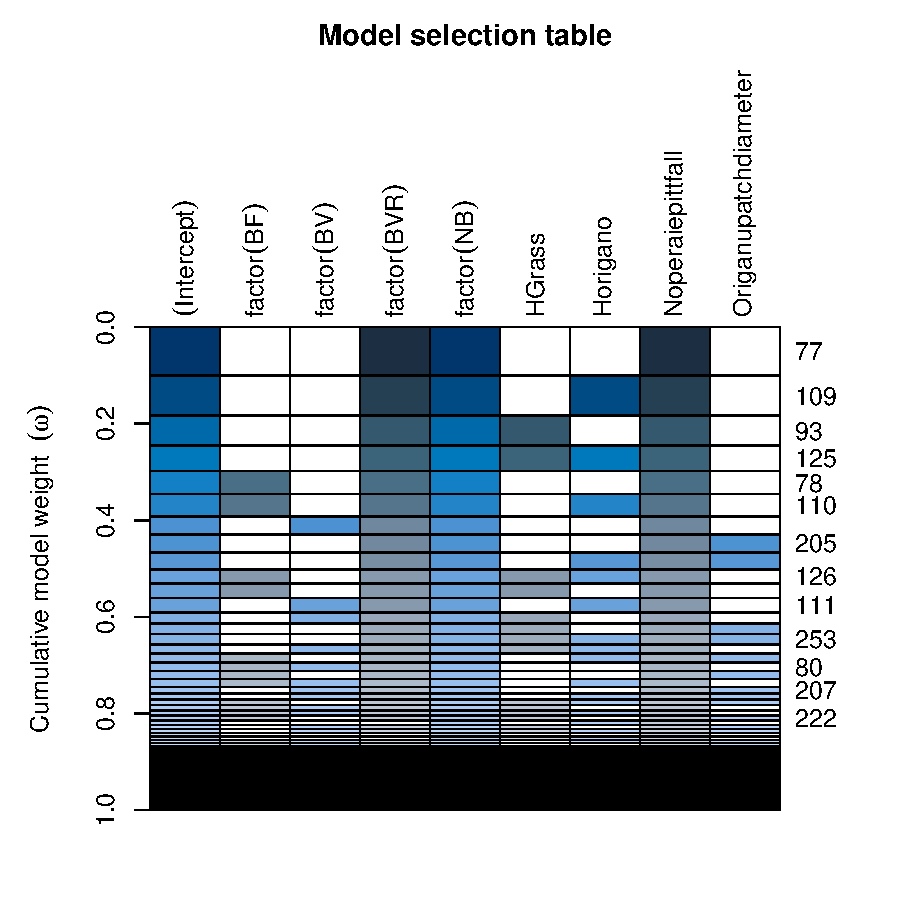
\includegraphics[height=0.8\textheight,keepaspectratio=false]{pictures/Rplot-glm-modelselectionplot.pdf}
\end{figure}

\end{frame}


% %------------------------------------------------
% \begin{frame}[fragile]
% \frametitle{Model selection: model averaging}
% 
% <<label=glm-modelselection-averagecoef, echo=FALSE, fig=TRUE, include=FALSE>>=
% 
% # Model average models with delta AICc < 2
% model.avg(dd, subset = delta < 2)$coefficients[,c(1:4)]
% model.avg(dd, subset = delta < 2)$coefficients[,c(5:7)]
% model.avg(dd, subset = delta < 2)$coefficients[,c(8:9)]
% #or as a 95% confidence set:
% # model.avg(dd, subset = cumsum(weight) <= .95) # get averaged coefficients
% 
% @
% 
% \end{frame}

% %------------------------------------------------
% \begin{frame}[fragile]
% \frametitle{Model selection: best model}
% 
% <<label=glm-bestmodel, echo=FALSE>>=
% 
% #'Best' model
% summary(get.models(dd, 1)[[1]])$coef
% 
% @
% 
% \end{frame}


% %------------------------------------------------
% \begin{frame}[fragile]
% \frametitle{Diagnostics - best model}
% 
% \begin{center}
% Binomial diagnostics are crazy!\\
% \end{center}
% 
% <<label=glm-diagnostics, eval=TRUE, fig=TRUE, include=FALSE, echo=FALSE>>=
% 
% op <- par(mfrow=c(2,2))
% plot(get.models(dd, 1)[[1]])
% par(op)
% 
% @
% 
% \begin{figure}
% 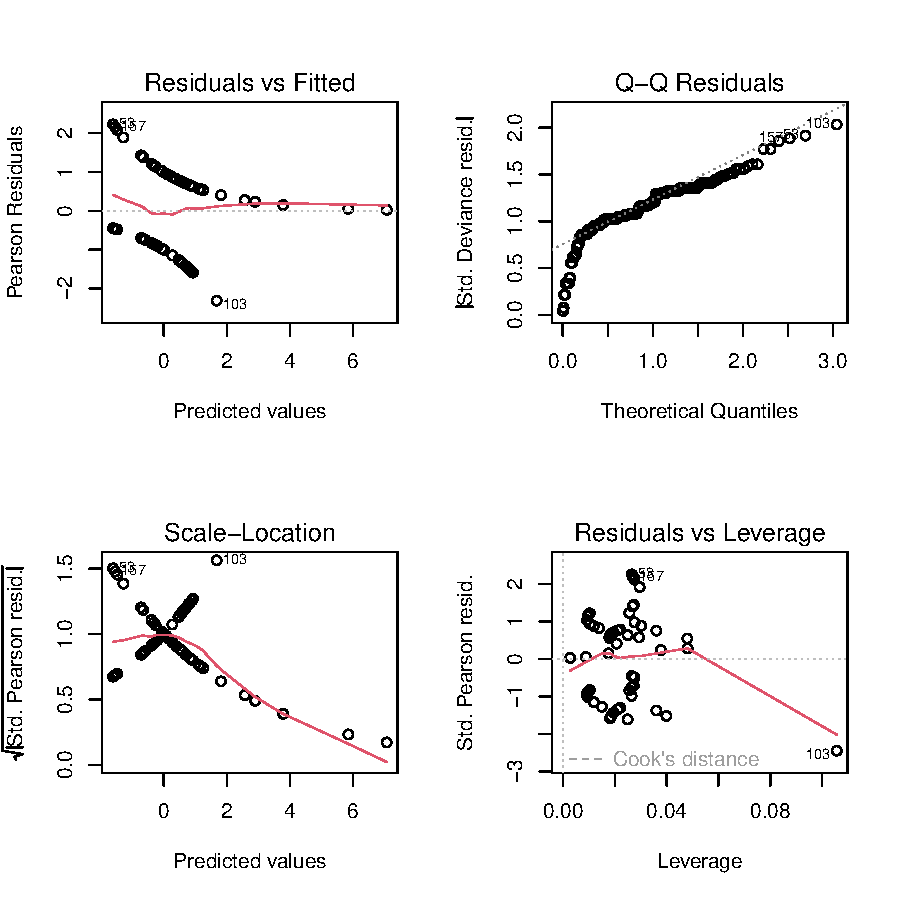
\includegraphics[height=0.8\textheight,keepaspectratio=false]{pictures/Rplot-glm-diagnostics.pdf}
% \end{figure}
% 
% \end{frame}

%------------------------------------------------
\section{Correlation structure} % Sections can be created in order to organize your presentation into discrete blocks, all sections and subsections are automatically printed in the table of contents as an overview of the talk
%------------------------------------------------

\subsection{Repeated observations} % A subsection can be created just before a set of slides with a common theme to further break down your presentation into chunks

\begin{frame}[fragile]
\frametitle{Introducing the Specimen - exercise 3}


\begin{Schunk}
\begin{Sinput}
> dati.GLMM <- read.csv("dati/dati.GLMM.csv")
> str(dati.GLMM)
\end{Sinput}
\begin{Soutput}
'data.frame':	214 obs. of  14 variables:
 $ X                   : int  1 2 3 4 5 6 7 8 9 10 ...
 $ id                  : int  1 2 3 4 5 6 7 8 9 10 ...
 $ Specimen            : int  1 6 4 5 5 6 8 8 8 8 ...
 $ Egg10               : int  0 0 0 0 0 0 0 0 0 0 ...
 $ MyrmicaYN           : int  0 0 0 0 0 0 0 0 0 0 ...
 $ Noperaiepittfall    : int  0 0 0 0 0 0 0 0 0 0 ...
 $ Horigano            : num  50 50 30 60 70 37.5 50 45 25 55 ...
 $ HGrass              : int  10 10 10 40 15 15 10 15 15 5 ...
 $ Origanupatchdiameter: int  50 50 3 60 190 50 120 90 15 25 ...
 $ BV                  : int  0 0 1 1 1 0 1 1 1 1 ...
 $ BVR                 : int  0 0 0 0 0 0 0 0 0 0 ...
 $ BR                  : int  1 1 0 0 0 1 0 0 0 0 ...
 $ BF                  : int  1 1 0 0 0 1 0 0 0 0 ...
 $ NB                  : int  0 0 0 0 0 0 1 0 1 0 ...
\end{Soutput}
\begin{Sinput}
> 
\end{Sinput}
\end{Schunk}



\end{frame}

%------------------------------------------------

\begin{frame}[fragile]
\frametitle{Repeated observations, are they a nuisance?}

\begin{columns}

\column{0.6\textwidth}
Repeated observations on the same individuals are often assumed to give rise to constant within group correlation structures.\\
\vspace{0.5cm}
% \onslide<2->{
Even if we assume independence among observations taken on different individuals, there will probably be a (constant?) {\bf correlation between any two observations from the same individual}.\\
% }

\column{0.4\textwidth}
% \onslide<2->{
\begin{figure}
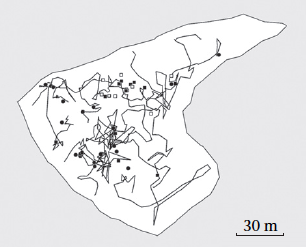
\includegraphics[width=0.8\linewidth]{pictures/trajectory}
\end{figure}
% }

\end{columns}
\end{frame}


%------------------------------------------------

\begin{frame}[fragile]
\frametitle{Repeated observations, are they a nuisance?}

\begin{columns}

\column{0.6\textwidth}
We can easily generalize to {\bf hierarchically structured populations}\\
\begin{itemize}
\item constant correlation among observations from the same individual
\item correlation to a lesser degree among observation from animals in the same herd
\item independence among observations from animals in different herds
\end{itemize}

\column{0.4\textwidth}
\begin{figure}
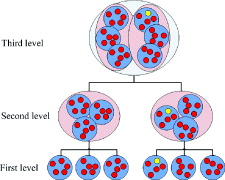
\includegraphics[width=0.8\linewidth]{pictures/livelli}
\end{figure}

\end{columns}
\end{frame}


%------------------------------------------------

\begin{frame}[fragile]
\frametitle{Correlation vs. autocorrelation}

\begin{block}{Correlation}
It is due to the hierarchical nature of data, and it results in general correlation structures
\end{block}

\begin{block}{Autocorrelation}
Specifically, the within-animal correlation patterns (eg. correlations that change as a function of temporal and spatial distance between observations)
\end{block}


\end{frame}

%------------------------------------------------

\begin{frame}[fragile]
\frametitle{Correlation structure: assumptions}

\begin{center}
Animals are randomly sampled and
independence is assumed among observations taken on different individuals
% \onslide<2->{
\begin{figure}
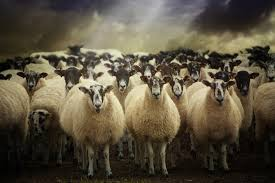
\includegraphics[width=0.8\linewidth]{pictures/sheep}
\end{figure}
% }
\end{center}

\end{frame}


%------------------------------------------------

\subsection{Implications}

\begin{frame}[fragile]
\frametitle{Issues}

Correlation violates the assumption of independence\begin{itemize}
\item biased estimates of coefficients
\item deceptively low estimates of uncertainty
\item overfit models
\item spurious conclusion!!
\end{itemize}

\begin{center}
In our previous analysis, the relocation was considered as the experimental unit, but we actually pooled data across animals.\\
\vspace{0.5cm}
POOLING HAS IMPORTANT CONSEQUENCES FOR INFERENCE
\end{center}

\end{frame}



%------------------------------------------------
\begin{frame}[fragile]
\frametitle{Issues}

Pooling observations from several animals is often the {\bf only option} when sample size is limited. But we are violating the assumption of independence\ldots (this constitutes pseudo-replication)\\
\vspace{0.5cm}
Three main avenues:\begin{enumerate}
\item data censoring - collect data a priori (or rarify through subsampling) to satisfy the assumption of independence
\item variance inflation - adopt a post hoc approach to adjust (inflate) standard errors of the parameters
\item explicit modelling of correlation
\end{enumerate}
\vspace{0.5cm}
When sample size is sufficient (for both the no. of animals and no. of relocations per animal), {\bf animals (not relocations) should be considerd as the unit of replication if we want to infer average selection patterns for the entire population}

\end{frame}


%------------------------------------------------

\section{Explicit modelling of correlation}
\subsection{Two-stage methods}

\begin{frame}[fragile]
\frametitle{An intuitive approach}

\begin{block}{First stage}
Regression models may be fit to data from individual animals and then averaged to determine population level responses.\\
$$ Y_{ij} = \alpha_i + \beta_i x_{ij} + \epsilon_{ij} $$\\
We obtain 22 estimates of $\alpha_i$ and $\beta_i$
\end{block}

% \onslide<2->{
\begin{block}{Second stage}
Sample means and variances are used in the second stage to characterize population means and variances.\\
\end{block}
% }

\end{frame}


% %------------------------------------------------
% \begin{frame}[fragile]
% \frametitle{Two-stage method: averaging}
% 
% To make statistical inference to the population, coefficients (or odd ratios) can be averaged across the set of sample animals. {\bf This approach effectively uses the animal as the experimental unit}. The average coefficient fo the {\it j}th variable:
% 
% $$ \beta_{.j} = \sum\limits_{i=1}^n \beta_{ij} $$
% 
% where $\beta_{ij}$ is the logistic regression coefficient for the {\it i}th animal and the {\it j}th variable.\\
% 
% The standard error for this estimate is:
% 
% $$ se(\beta_{.j}) = \sqrt{\frac{\sum\limits_{i=1}^n (\beta_{ij}-\beta_j)^2}{n-1}/n}$$
% 
% 
% \end{frame}


% %------------------------------------------------
% \begin{frame}[fragile]
% \frametitle{Two-stage method: variance}
% 
% \begin{columns}
% \column{0.4\textwidth}
% Variance estimators will be biased high, unless the sampling uncertainty associated with individual $\hat{\beta}_i$ is accounted for.
% 
% \column{0.6\textwidth}
% \begin{figure}
% 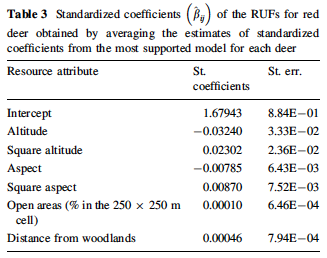
\includegraphics[width=0.8\linewidth]{pictures/LETable3}
% \end{figure}
% 
% \end{columns}
% 
% \end{frame}


%------------------------------------------------
\begin{frame}[fragile]
\frametitle{Two-stage method: advantages}

\begin{itemize}
\item unbiased estimators of $\bar{\beta}$ assuming individuals are independent
\item can determine different covariate structures for each individual (model selection at individual level)
\item model selection can be performed at the population level (makes more sense if we want to characterize typical selection patterns - note: likelihoods are additive given independence of the animals)
\end{itemize}

\end{frame}

%% exercise 3

%------------------------------------------------
\begin{frame}[fragile]
\frametitle{Two-stage method: drawbacks}

\begin{itemize}
\item sufficient data must exist for fitting individual-level models
\end{itemize}

\begin{Schunk}
\begin{Soutput}
[1] 22
\end{Soutput}
\end{Schunk}


\begin{Schunk}
\begin{Sinput}
> table(dati.GLMM$Specimen)
\end{Sinput}
\begin{Soutput}
 1  2  3  4  5  6  7  8  9 10 12 13 14 15 16 17 18 19 20 21 22 23 
 4  2  5  9  9 12 13 19  3 27 31 10 12  2  5  9  9  2  7 17  4  3 
\end{Soutput}
\begin{Sinput}
> 
\end{Sinput}
\end{Schunk}

Are we going to drop individuals that are followed for only a short period of time?
%' Data become less representative
%' 
%' 
%' 
%' when sufficient data have been collected to allow effcient estimation of individual-specific regression parameters
%' 
%' 
%' Advantages:

\end{frame}

%------------------------------------------------

%\section{Explicit modelling of correlation}
\subsection{Mixed-effects models}

\begin{frame}[fragile]
\frametitle{Random effects - exercise 4}

With the two-stage approach, the animal is treated as a {\bf random effect}.\\
\vspace{0.5cm}

A variable is considered random when the investigator has not controlled explicitly for levels of the variable in the experimental design, but {\bf has chosen a random sample of levels from the population}

\begin{center}
\begin{figure}
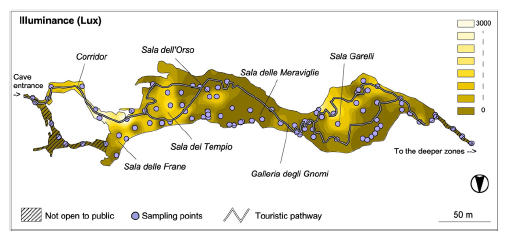
\includegraphics[width=0.8\linewidth]{pictures/samplingpoints}
\end{figure}
\end{center}

\end{frame}


%------------------------------------------------

%\section{Explicit modelling of correlation}
%\subsection{Mixed-effects models}

\begin{frame}[fragile]
\frametitle{Mixed model formulation}

By including a random effect for individuals, individual variability is identified explicitly and the scope of inference can be extended to the entire population\\
\vspace{0.5cm}
Mixed-effects models offer a powerful apporach to modelling correlated data under the assumption that latent or unmeasured characteristics associated with individuals might induce correlation among repeated measurements on these individuals.

$$ {\bf Y = X\beta + Zb + \epsilon} $$

% Please note: in a mixed model, we do have two variance-covariance matrices (one for the error, as in simple regression model, and one for the random factors!)\\

\end{frame}


%------------------------------------------------
%\section{Explicit modelling of correlation}
%\subsection{Mixed-effects models}

% \begin{frame}[fragile]
% \frametitle{Mixed model assumption}
% 
% \begin{center}
% $$ b_i \tilde N(0,D) $$
% $$ \epsilon \tilde N(0,\sum) $$
% \vspace{0.5cm}
% $b_1$, \ldots, $b_N$, $\epsilon_1$, \ldots, $\epsilon_N$ are independent
% \end{center}
% 
% \end{frame}


% %------------------------------------------------
% %\section{Explicit modelling of correlation}
% %\subsection{Mixed-effects models}
% 
% \begin{frame}[fragile]
% \frametitle{Random intercept model}
% 
% Reminder! We use a typical fixed-effects exponential resource selection function:
% $$ \hat{w}(x) = exp(\hat{\beta}_0 + \hat{\beta}_1 x_1 + \hat{\beta}_2 x_2 + ... + \hat{\beta}_n x_n) $$ 
% Parameters are estimated from logistic regression.\\
% \vspace{0.5cm}
% For a random intercept model, the logit model $g(x)$:
% 
% $$ g(x) = \beta_0 + \beta_1 x_{1ij} + \beta_2 x_{2ij} + ... + \beta_n x_{nij} + \gamma_{0j} $$
% 
% $\gamma_{0j}$ is the random intercept, which is the difference between the mean intercept $\beta_0$ for all groups and the intercept for group {\it j}
% 
% 
% \end{frame}



%------------------------------------------------
%\section{Explicit modelling of correlation}
%\subsection{Mixed-effects models}

\begin{frame}[fragile]
\frametitle{Random intercept model: interpretation}

For a single animal, the logit model $g(x)$ is:

$$ g(x) = (\beta_0 + \gamma_{0j}) + \beta_1 x_{1ij} + \beta_2 x_{2ij} + ... + \beta_n x_{nij}  $$

\begin{columns}
\column{0.6\textwidth}
\begin{figure}
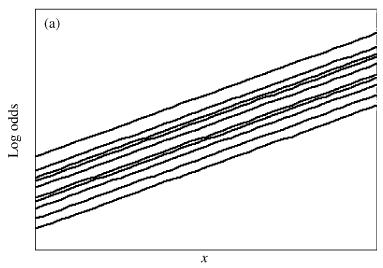
\includegraphics[width=0.8\linewidth]{pictures/randomintercept}
\end{figure}

\column{0.4\textwidth}
Random intercepts allow the intercept or magnitude of the response to vary among animals.\\
{\bf The addition of a random intercept compensates for unbalanced designs}
%L'effetto delle variabili è lo stesso su tutti gli animali, perché i coefficienti angolari non cambiano
\end{columns}

\end{frame}


%------------------------------------------------
%\section{Explicit modelling of correlation}
%\subsection{Mixed-effects models}

\begin{frame}[fragile]
\frametitle{Random slope model: interpretation}

$$ g(x) = \beta_0 + \beta_1 x_{1ij} + ... + \beta_n x_{nij} + \gamma_{nj} x_{nj} $$

\begin{columns}
\column{0.6\textwidth}
\begin{figure}
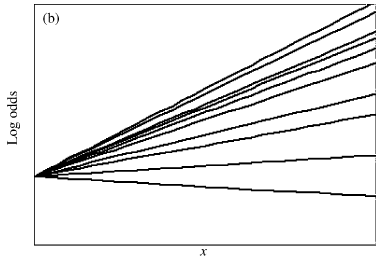
\includegraphics[width=0.8\linewidth]{pictures/randomslope}
\end{figure}

\column{0.4\textwidth}
\only<1>{The inclusion of random coefficients allows the effect of covariates to vary among animals. {\bf This is more biologically meaningfull}\\}
\only<2>{BUT\ldots what about the number of parameters??\\}
\only<3>{If we fit models with random coefficients, we allow for animal-level specific estimates for a response (conditional estimates) and for an overall estimate (marginal or population-level estimator)}

\end{columns}

\end{frame}

%------------------------------------------------
%\section{Explicit modelling of correlation}
%\subsection{Mixed-effects models}

\begin{frame}[fragile]
\frametitle{Random intercept and slope model: interpretation}

$$ g(x) = (\beta_0 + \gamma_{0j}) + \beta_1 x_{1ij} + ... + \beta_n x_{nij} + \gamma_{nj} x_{nj} $$

% \begin{columns}
% \column{0.6\textwidth}
\begin{figure}
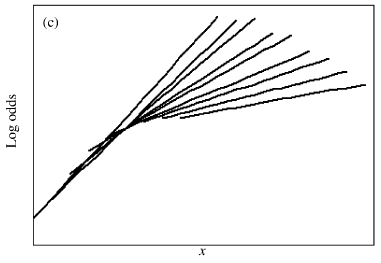
\includegraphics[width=0.8\linewidth]{pictures/randominterceptandslope}
\end{figure}

% \column{0.4\textwidth}

% \end{columns}

\end{frame}


%------------------------------------------------
%\section{Explicit modelling of correlation}
%\subsection{Mixed-effects models}

\begin{frame}[fragile]
\frametitle{R packages}

\begin{figure}
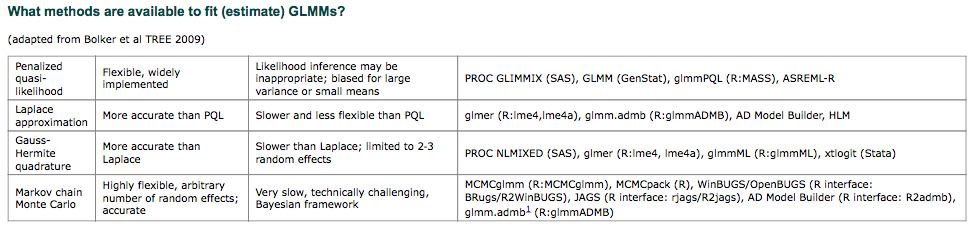
\includegraphics[width=1.2\linewidth]{pictures/Rpackages}
\end{figure}

\end{frame}

%------------------------------------------------
%\section{Explicit modelling of correlation}
%\subsection{Mixed-effects models}

\begin{frame}[fragile]
\frametitle{Mixed model selection}


\begin{figure}
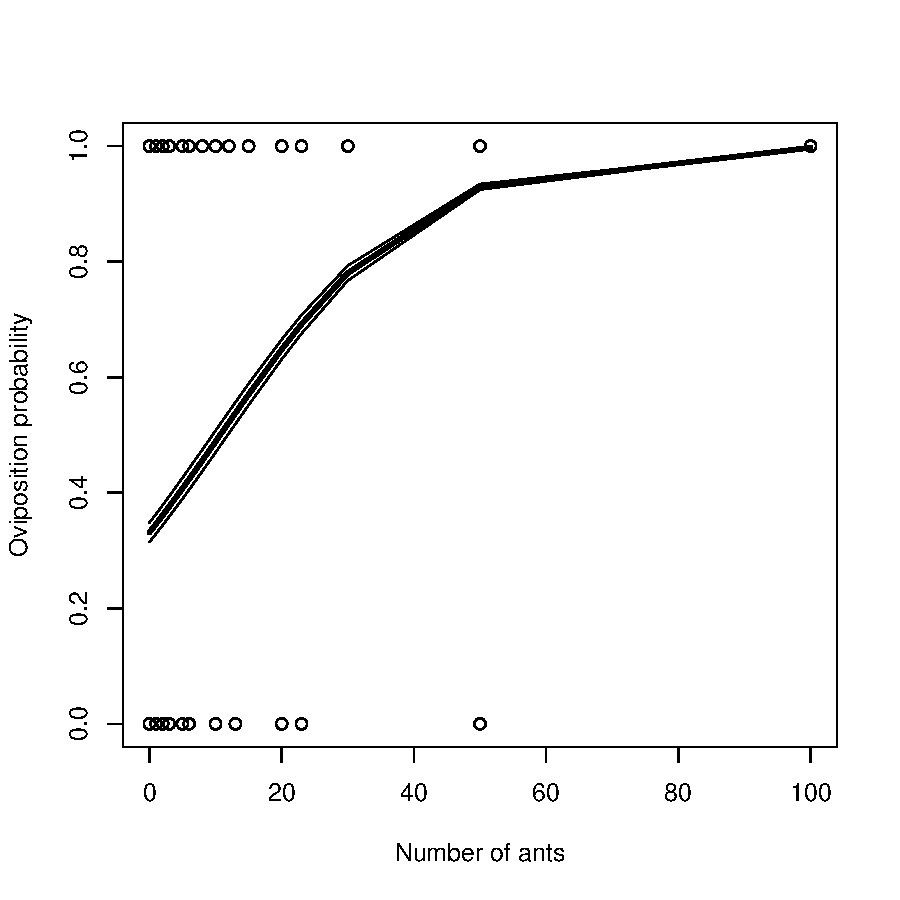
\includegraphics[width=0.6\textwidth]{pictures/Rplot-representation.pdf}
\end{figure}

\end{frame}



%------------------------------------------------
%\section{Explicit modelling of correlation}
%\subsection{Mixed-effects models}

\begin{frame}[fragile]
\frametitle{Any other issue?}

\begin{figure}
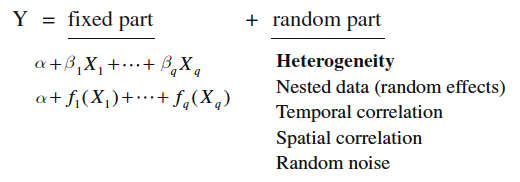
\includegraphics[width=1\textwidth]{pictures/otherissues}
\end{figure}

\end{frame}




%------------------------------------------------
%\section{Explicit modelling of correlation}
%\subsection{Mixed-effects models}

\begin{frame}[fragile]
\frametitle{Mixed models for resource selection: advantages}

Mixed-effects models are appealing

\begin{itemize}
\item they match the way in which ecological data are structured
\item they can effectively use data from individuals having few data points, eliminating the problem of sampling inequities among individuals
\item they simultaneously fit individual- and population-level models, efficiently pooling information across individuals
\end{itemize}

\end{frame}

% %------------------------------------------------
% %\section{Explicit modelling of correlation}
% %\subsection{Mixed-effects models}
% 
% \begin{frame}[fragile]
% \frametitle{Mixed models for resource selection: disadvantages}
% 
% GLMMs are at the frontier of research\ldots
% 
% \begin{itemize}
% \item correctly specifying the correlation structure is challenging for use-availability designs (note: the correlation among pairs of used points is likely to differ from the correlation among used-available points - ASK FOR HELP!!)
% \item GLMMs can be computationally challenging to fit, requiring approximate likelihood techniques, numerical integration or Bayesian implementations using MCMC methods
% \item parameter estimates are sensitive to the choice of the methods
% \item for GLMMs using a logit link, Gaussian adaptive quadrature is advised, but it is computationally intensive and numerical integration approaches can fail to converge
% \end{itemize}
% 
% \end{frame}



%------------------------------------------------
%\section{Explicit modelling of correlation}
%\subsection{Mixed-effects models}

\begin{frame}[fragile]
\frametitle{Main references}

\begin{itemize}
\item Manly et al 2002 Resource selection by animals. Statistical design and analysis for field studies. Kluwer Academic Publisher
\item Millspaugh \& Marzluff (eds) 2001 Radio tracking and animal populations. Academic Press.
\item Gillies et al 2006 Application of random effects to the study of resource selection by animals. Journal of Animal Ecology 75:887-898
\item Fieberg et al 2010 Correlation and studies of habitat selection: problem, red herring or opportunity? Philophical Transactions of the Royal Society B 365:2233-2244
\item Burnham \& Anderson 2002 Model Selection and Multimodel Inference. A Practical Information-Theoretic Approach. Springer.
\item Zuur et al 2009 Mixed effects models and extensions in ecology with R. Springer
\end{itemize}

\end{frame}


%------------------------------------------------

\begin{frame}
\frametitle{Overview} % Table of contents slide, comment this block out to remove it
\tableofcontents % Throughout your presentation, if you choose to use \section{} and \subsection{} commands, these will automatically be printed on this slide as an overview of your presentation
\end{frame}




\end{document}

